%%%%%%%%%%%%%%%%%%%%%%%%%%%%%%%%%%%%%%%%%%%%%%%%%%%%%%%%%%%%%%%%%%%%%%%%%%%%%%%%%%%%%
% Fundamental Current i^1_1 and fundamental volage u^1_2 for single-phase DC inverter
%%%%%%%%%%%%%%%%%%%%%%%%%%%%%%%%%%%%%%%%%%%%%%%%%%%%%%%%%%%%%%%%%%%%%%%%%%%%%%%%%%%%%
\begin{figure}[h]

    %   \documentclass{standalone}
    %   \usepackage{pgfplots}
    %   \pgfplotsset{compat=1.18} % Kompatibilität für neuere Versionen
           \centering
           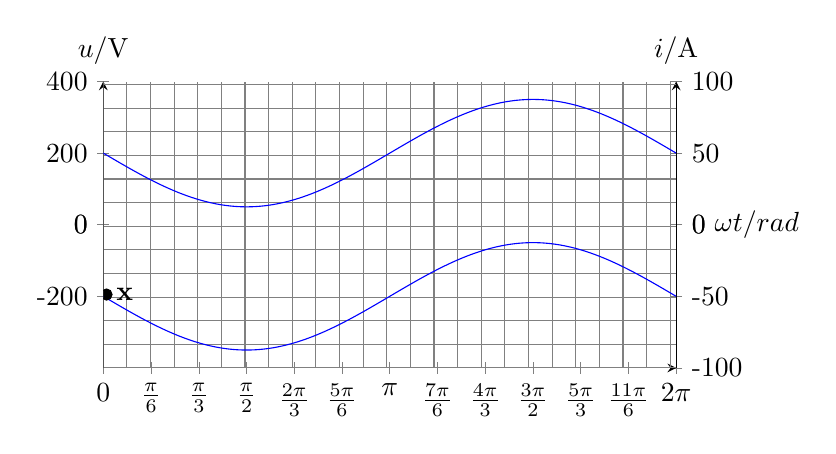
\begin{tikzpicture}
                \pgfplotsset{set layers}
           \begin{axis}[
            % x/y range adjustment
            scale only axis,
            ymin=-400, ymax=400,
            xmin=0, xmax=540, 
            samples=500,
            axis y line=center,
            axis x line=bottom,
            extra y ticks=0,
            % Label text
            xlabel={$\omega t / \text{rad}$},
            ylabel={$u/\mathrm{V}$},
            % Label adjustment
            x label style={at={(axis description cs:1.05,0.5)},anchor=west},
            y label style={at={(axis description cs:0,.97)},anchor=south,yshift=0.2cm},
            width=0.6\textwidth,
            height=0.3\textwidth,
            % x-Ticks
            xtick={0, 45, 90, 135, 180, 225, 270, 315, 360, 405, 450,495, 540},
            xticklabels={0, $\frac{\pi}{6}$,$\frac{\pi}{3}$, $\frac{\pi}{2}$, $\frac{2\pi}{3}$, $\frac{5\pi}{6}$, $\pi$, $\frac{7\pi}{6}$, $\frac{4\pi}{3}$, $\frac{3\pi}{2}$, $\frac{5\pi}{3}$, $\frac{11\pi}{6}$, $2\pi$},
            xticklabel style = {anchor=north},
            % y-Ticks
            ytick={-400,-200,0,200,400},
            yticklabels={-400,-200,0,200,400},
            yticklabel style = {anchor=east},
            % Grid layout
           % grid,
            %grid style={line width=.1pt, draw=gray!10},
            %major grid style={line width=.2pt,draw=gray!90},
        ] 
        % Grid
        \draw[step=0.3cm, gray, thin] (0,-400) grid (540,400);
        % internal load voltage u
        \addplot[blue, domain= 0:540, solid] {-150*sin(x/1.5)+200};
        \addplot[blue, domain= 0:540, solid] {-150*sin(x/1.5)-200};
         % Label of u
        % \node[black, fill=white, inner sep = 1pt, anchor = south] at (axis cs:120,160) {$u_{2\mathrm{i}}(t)$};
         % Start point
         \filldraw[black] (3,-195) circle (2pt) node[anchor=west]{\textbf{x}};
           \end{axis}
           \begin{axis}[
            % x/y range adjustment
            scale only axis,
            ymin=-100, ymax=100,
            xmin=0, xmax=360,
            axis x line=none, 
            samples=500,
            axis y line=right,
            axis x line=middle,
            extra y ticks=0,
            % Label text
            ylabel={$i/\mathrm{A}$},
            % Label adjustment
            y label style={rotate = -90,at={(axis description cs:1,.97)},anchor=south,yshift=0.2cm},
            width=0.6\textwidth,
            height=0.3\textwidth,
            % y-Ticks
            ytick={-100,-50,0,50,100},
            yticklabels={-100,-50,0,50,100},
            yticklabel style = {anchor=west},
            % Grid layout
           % grid,
            %grid style={line width=.1pt, draw=gray!10},
            %major grid style={line width=.2pt,draw=gray!90},
        ]
           \end{axis}             
           \end{tikzpicture}
           \caption{Harmonics of the output voltage and current.}
           \label{sfig:ex07_sub1.3_Harmonics}
   \end{figure}